\tikzstyle{cat1} = [rectangle, rounded corners, minimum width=3cm, minimum height=1cm, text centered, text width=3cm, draw=black, fill=black!0]
\tikzstyle{cat2} = [rectangle, minimum width=3cm, minimum height=1cm, text centered, text width=3cm, draw=black,  fill=black!10]
\tikzstyle{cat3} = [rectangle, minimum width=5cm, text centered, text width=5cm, minimum height=1cm, draw=black,  fill=black!10]

\tikzstyle{arrow} = [thick,->,>=stealth]

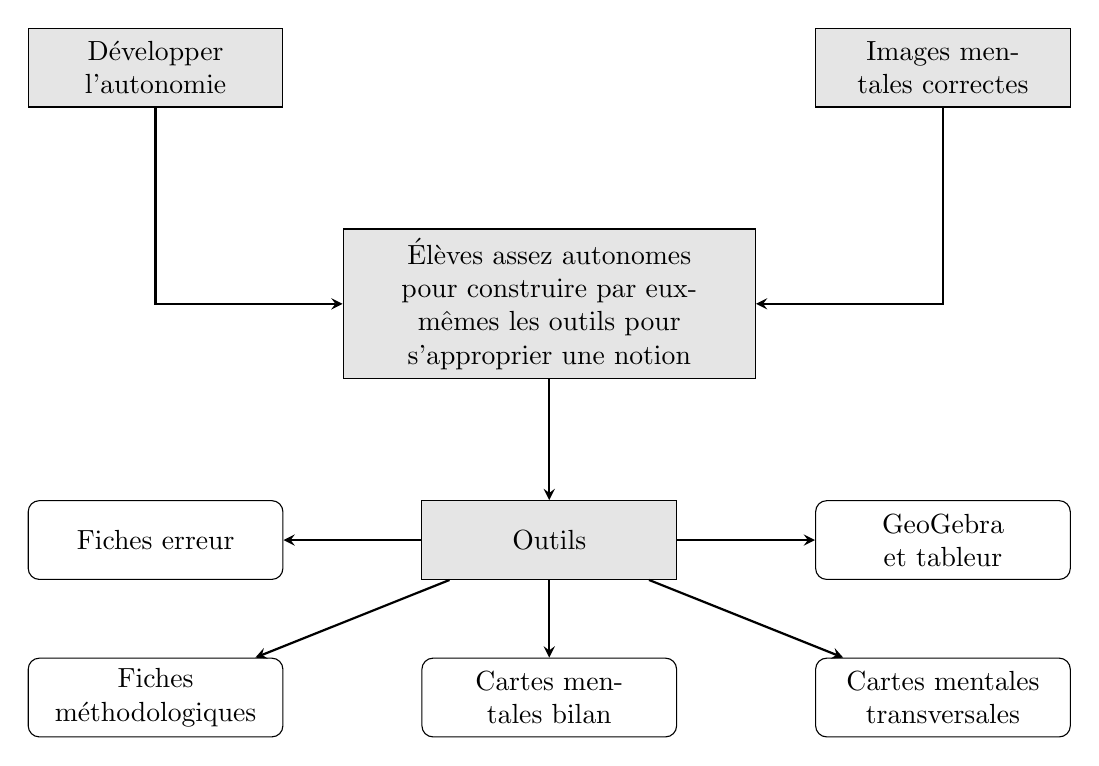
\begin{tikzpicture}[node distance=3cm]
\node (auto) [cat2] {Développer l'autonomie};
\node (img) [cat2, right of=auto, xshift=7cm] {Images mentales correctes};
\node (pb) [cat3, below of=auto, xshift=5cm] {Élèves assez autonomes pour construire par eux-mêmes les outils pour s'approprier une notion};
\node (outils) [cat2, below of=pb] {Outils};
\draw [arrow] (auto) |- (pb);
\draw [arrow] (img) |- (pb);
\draw [arrow] (pb) -- (outils);
\node (fiche1) [cat1, left of=outils, xshift=-2cm] {Fiches erreur};
\node (fiche2) [cat1, below of=outils, xshift=-5cm, yshift=1cm] {Fiches méthodologiques};
\node (carte1) [cat1, below of=outils, yshift=1cm] {Cartes mentales bilan};
\node (geogebra) [cat1, right of=outils, xshift=2cm] {GeoGebra et tableur};
\node (carte2) [cat1, below of=outils, xshift=5cm, yshift=1cm] {Cartes mentales transversales};
\draw [arrow] (outils) -- (fiche1);
\draw [arrow] (outils) -- (fiche2);
\draw [arrow] (outils) -- (geogebra);
\draw [arrow] (outils) -- (carte1);
\draw [arrow] (outils) -- (carte2);
\end{tikzpicture}
